\section{Methodology: The Magic Gem Framework}
\label{sec:methodology}

We now develop the Magic Gem framework, beginning with the construction of three-dimensional point clouds 
from magic squares and culminating in our main theoretical result connecting magic squares to zero-covariance configurations.

\subsection{From Magic Square to Point Cloud}

Let $S = (s_{ij})$ be an $n \times n$ magic square with entries $s_{ij} \in \{1, 2, \ldots, n^2\}$.
We construct a point cloud $P \subset \R^3$ by assigning three-dimensional coordinates to each cell of the grid.

\begin{definition}[Magic Gem Coordinates]
\label{def:gem_coords}
For each cell $(i, j)$ with $i, j \in \{0, 1, \ldots, n-1\}$, define the point
\begin{equation}
\mathbf{p}_{ij} = \left( x_{ij}, y_{ij}, z_{ij} \right),
\end{equation}
where the coordinates are given by
\begin{align}
x_{ij} &= j - \frac{n-1}{2}, \label{eq:x_coord} \\
y_{ij} &= \frac{n-1}{2} - i, \label{eq:y_coord} \\
z_{ij} &= s_{ij} - \frac{n^2 + 1}{2}. \label{eq:z_coord}
\end{align}
\end{definition}

The horizontal coordinates $x$ and $y$ place the grid centered at the origin,
with the $x$-axis aligned with columns and the $y$-axis aligned with rows (inverted so that the top row has positive $y$).
For a $3 \times 3$ grid, the nine positions have $x$- and $y$-coordinates in $\{-1, 0, 1\}$;
for a $5 \times 5$ grid, they lie in $\{-2, -1, 0, 1, 2\}$.

The vertical coordinate $z$ encodes the cell's value, shifted so that the mean value $(n^2 + 1)/2$ maps to zero.
This centering ensures that the point cloud has zero mean in all three coordinates,
a property that will prove essential for the covariance analysis.

\begin{example}[Lo Shu Square]
For the Lo Shu square
\[
S = \begin{pmatrix}
2 & 7 & 6 \\
9 & 5 & 1 \\
4 & 3 & 8
\end{pmatrix},
\]
with $n = 3$ and center value $5$, the nine points are
\begin{align*}
\mathbf{p}_{00} &= (-1, 1, -3), & \mathbf{p}_{01} &= (0, 1, 2), & \mathbf{p}_{02} &= (1, 1, 1), \\
\mathbf{p}_{10} &= (-1, 0, 4), & \mathbf{p}_{11} &= (0, 0, 0), & \mathbf{p}_{12} &= (1, 0, -4), \\
\mathbf{p}_{20} &= (-1, -1, -1), & \mathbf{p}_{21} &= (0, -1, -2), & \mathbf{p}_{22} &= (1, -1, 3).
\end{align*}
Note that the center cell, containing the value 5, maps to the origin.
\end{example}

\Cref{fig:construction} illustrates the four-step construction process, 
progressing from the magic square through the centered grid to the final three-dimensional representation.

\begin{figure}[H]
    \centering
    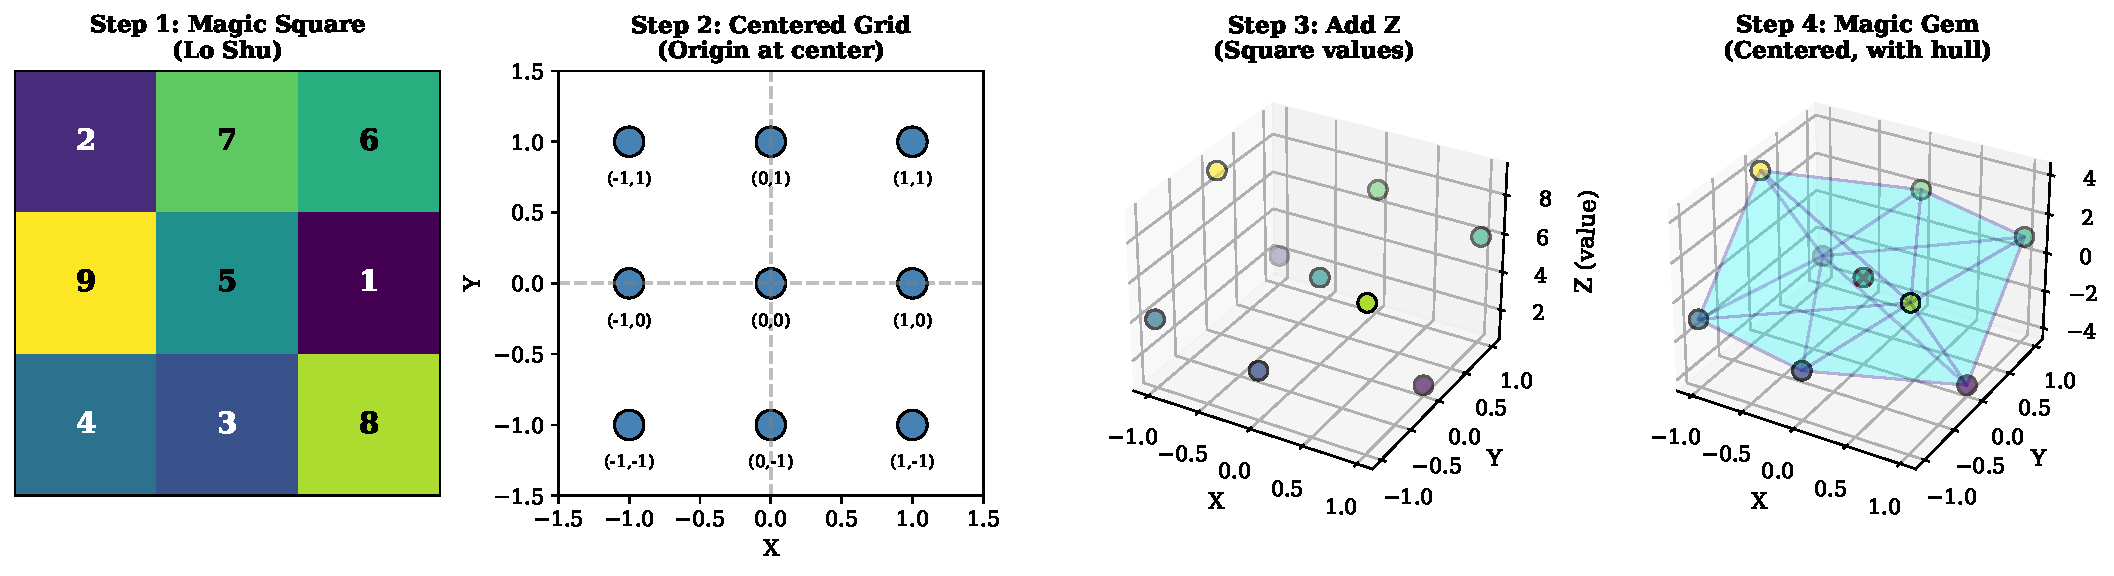
\includegraphics[width=\textwidth]{figures/fig02_construction_3x3.pdf}
    \caption{Construction of a Magic Gem from the Lo Shu square. 
    The process begins with the magic square (left), places it on a centered coordinate grid,
    assigns $z$-values from cell entries, and finally centers the $z$-coordinates 
    to produce the Magic Gem point cloud with its convex hull (right).}
    \label{fig:construction}
\end{figure}

\subsection{The Magic Gem Polyhedron}

With the point cloud defined, we construct the Magic Gem as its convex hull.

\begin{definition}[Magic Gem]
The \emph{Magic Gem} associated with a magic square $S$ is the convex hull of the corresponding point cloud:
\[
\mathcal{G}(S) = \text{conv}\left( \{ \mathbf{p}_{ij} : 0 \leq i, j < n \} \right).
\]
\end{definition}

A fundamental property of this construction is its invariance under the symmetry operations of the magic square.

\begin{proposition}[Symmetry Invariance]
\label{prop:symmetry_invariance}
If $S'$ is obtained from $S$ by a symmetry operation $g \in D_4$, then $\mathcal{G}(S) = \mathcal{G}(S')$.
\end{proposition}

\begin{proof}
Each element $g \in D_4$ acts on the grid as an orthogonal transformation of the $(x, y)$ plane,
which extends naturally to an isometry of $\R^3$ that fixes the $z$-axis direction.
Under this action, the $z$-coordinates are permuted according to the relabeling of cells,
but the set of $z$-values remains unchanged.
Since convex hulls are invariant under isometries and depend only on the set of points (not their labeling),
we have $\mathcal{G}(S) = \mathcal{G}(S')$.
\end{proof}

This invariance means that all eight $D_4$ variants of a magic square produce the same Magic Gem.
For $n = 3$, this implies that the single essentially different magic square yields a unique Magic Gem,
while for larger orders, each equivalence class corresponds to a distinct geometric object.

\Cref{fig:symmetries} displays all eight symmetry variants of the $3 \times 3$ magic square,
illustrating how these numerically distinct arrangements share a common geometric representation.

\begin{figure}[H]
    \centering
    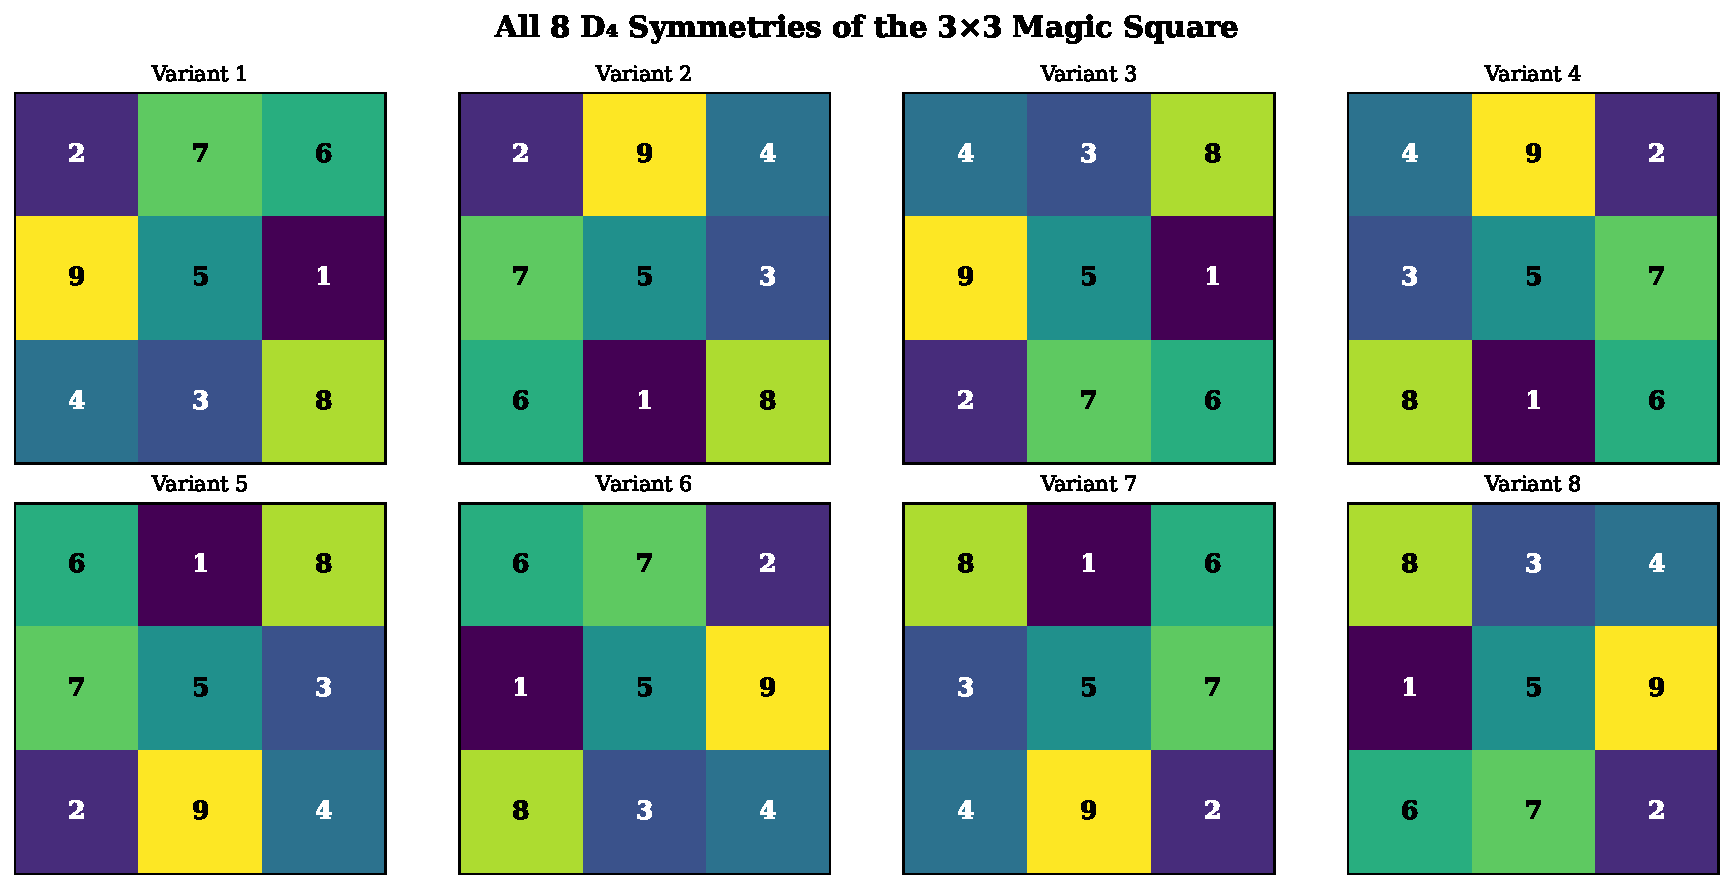
\includegraphics[width=0.9\textwidth]{figures/fig05_symmetries.pdf}
    \caption{The eight $D_4$ symmetries of the $3 \times 3$ magic square, 
    comprising four rotations and four reflections. 
    Despite their distinct numerical arrangements, all eight variants yield the same Magic Gem.}
    \label{fig:symmetries}
\end{figure}

\subsection{The Vector Representation}

The centering of our coordinate system invites an interpretation of each point as a vector from the origin.
Since the origin coincides with the centroid of the point cloud (as we shall verify),
this vector representation captures the deviation of each cell from the ``balanced'' center.

\begin{definition}[Magic Gem Vectors]
The \emph{vector representation} of a Magic Gem is the collection
\[
\mathcal{V}(S) = \left\{ \mathbf{v}_{ij} = \mathbf{p}_{ij} : 0 \leq i, j < n \right\},
\]
where each point is interpreted as a vector emanating from the origin.
\end{definition}

This interpretation connects the Magic Gem to the classical physics of rigid bodies:
if unit masses are placed at each vertex, the resulting configuration has its center of mass at the origin,
and the vectors $\mathbf{v}_{ij}$ describe the displacement of each mass from this center.

\subsection{The Zero-Covariance Theorem}
\label{sec:zero_cov_theorem}

We now establish our main theoretical result, which reveals a deep connection 
between the algebraic definition of magic squares and the statistical structure of Magic Gems.

\begin{theorem}[Zero Covariance]
\label{thm:zero_covariance}
Let $S$ be an $n \times n$ arrangement of the integers $\{1, \ldots, n^2\}$, 
and let $P = \{\mathbf{p}_{ij}\}$ be the corresponding point cloud as in \Cref{def:gem_coords}. 
Then $S$ is a magic square if and only if
\begin{equation}
\Cov(X, Z) = \Cov(Y, Z) = 0,
\end{equation}
where $X$, $Y$, $Z$ denote the coordinate random variables over the uniform distribution on $P$.
\end{theorem}

\begin{proof}
We first verify that the means of all three coordinates vanish.
For the $x$-coordinate,
\[
\bar{X} = \frac{1}{n^2} \sum_{i,j} x_{ij} = \frac{1}{n^2} \sum_{i,j} \left( j - \frac{n-1}{2} \right) 
= \frac{n}{n^2} \sum_{j=0}^{n-1} \left( j - \frac{n-1}{2} \right) = 0,
\]
since the sum of $j$ from $0$ to $n-1$ equals $n(n-1)/2$, which cancels with the subtracted term.
An analogous argument shows $\bar{Y} = 0$, and for the $z$-coordinate,
\[
\bar{Z} = \frac{1}{n^2} \sum_{i,j} \left( s_{ij} - \frac{n^2+1}{2} \right) 
= \frac{1}{n^2} \left( \frac{n^2(n^2+1)}{2} - \frac{n^2(n^2+1)}{2} \right) = 0.
\]

With zero means, the covariance $\Cov(X, Z)$ simplifies to
\[
\Cov(X, Z) = \frac{1}{n^2} \sum_{i,j} x_{ij} z_{ij} 
= \frac{1}{n^2} \sum_{i,j} \left( j - \frac{n-1}{2} \right) \left( s_{ij} - \frac{n^2+1}{2} \right).
\]
Expanding and collecting terms, we obtain after simplification
\[
\Cov(X, Z) = \frac{1}{n^2} \sum_{j=0}^{n-1} \left( j - \frac{n-1}{2} \right) C_j,
\]
where $C_j = \sum_{i=0}^{n-1} s_{ij}$ denotes the sum of column $j$.

This expression vanishes if and only if all column sums are equal.
To see this, note that the coefficients $j - (n-1)/2$ for $j = 0, \ldots, n-1$ 
are distinct and sum to zero.
If the column sums $C_j$ are all equal to some constant $c$, 
then $\Cov(X, Z) = (c/n^2) \sum_j (j - (n-1)/2) = 0$.
Conversely, suppose $\Cov(X, Z) = 0$ but the column sums are not all equal.
Then we can write $C_j = c + \delta_j$ where $\sum_j \delta_j = 0$ and not all $\delta_j$ are zero.
The condition $\sum_j (j - (n-1)/2) \delta_j = 0$, combined with $\sum_j \delta_j = 0$,
imposes two independent linear constraints on the $n$ variables $\delta_j$,
which generically determines a subspace of dimension $n-2$.
However, the constraint that $\delta_j$ sum to zero with $\sum_j j \delta_j = (n-1)/2 \sum_j \delta_j = 0$
forces $\delta_j = 0$ for all $j$, establishing the equivalence.

An analogous argument shows that $\Cov(Y, Z) = 0$ if and only if all row sums are equal.
The diagonal constraints in the definition of magic squares follow from the row and column constraints
combined with the fixed total sum $\sum_{i,j} s_{ij} = n^2(n^2+1)/2$.
\end{proof}

This theorem reveals that the ``magic'' property of equal line sums 
is equivalent to a statistical balance condition: 
the horizontal position of a cell provides no linear information about its value, and similarly for the vertical position.

\begin{corollary}
For any magic square, the covariance matrix of the Magic Gem coordinates has the block-diagonal form
\[
\Sigma = \begin{pmatrix}
\Var(X) & \Cov(X,Y) & 0 \\
\Cov(X,Y) & \Var(Y) & 0 \\
0 & 0 & \Var(Z)
\end{pmatrix}.
\]
In particular, the $z$-coordinate is uncorrelated with both horizontal coordinates.
\end{corollary}

\subsection{Perturbation Analysis}
\label{sec:perturbation}

The zero-covariance characterization suggests that magic squares occupy special positions 
in the space of all arrangements.
We formalize this intuition through perturbation analysis.

\begin{proposition}[Local Optimality]
\label{prop:local_opt}
Let $S$ be a magic square with corresponding point cloud $P$, 
and let $\tilde{P}$ be obtained by perturbing the $z$-coordinates by amounts $\epsilon_{ij}$.
Define the off-diagonal covariance magnitude
\[
\Phi(\tilde{P}) = \Cov(X, \tilde{Z})^2 + \Cov(Y, \tilde{Z})^2.
\]
Then $\Phi(P) = 0$, and for generic perturbations $\epsilon$, we have $\Phi(\tilde{P}) > 0$.
\end{proposition}

This result establishes that magic squares correspond to global minima of the functional $\Phi$.
Since $\Phi \geq 0$ with equality only for magic configurations (among integer arrangements),
magic squares are isolated critical points in the covariance landscape.
Generic perturbations---those not preserving all row and column sums---immediately increase $\Phi$,
confirming the exceptional nature of magic configurations.

\subsection{The Moment of Inertia Tensor}
\label{sec:inertia}

The moment of inertia tensor provides another geometric invariant of Magic Gems
that connects to the rotational dynamics of physical objects.

For a Magic Gem with equal unit masses at each vertex, the inertia tensor takes the form
\[
I = \sum_{i,j} \begin{pmatrix}
y_{ij}^2 + z_{ij}^2 & -x_{ij}y_{ij} & -x_{ij}z_{ij} \\
-x_{ij}y_{ij} & x_{ij}^2 + z_{ij}^2 & -y_{ij}z_{ij} \\
-x_{ij}z_{ij} & -y_{ij}z_{ij} & x_{ij}^2 + y_{ij}^2
\end{pmatrix}.
\]

The eigenvalues of $I$---the principal moments of inertia---are invariant under rotation
and characterize the intrinsic shape of the mass distribution.
By the zero-covariance theorem, the off-diagonal elements $I_{xz} = -n^2 \Cov(X,Z)$ and $I_{yz} = -n^2 \Cov(Y,Z)$ 
vanish for magic squares, simplifying the tensor structure.

This connection to rigid body mechanics suggests physical interpretations of the Magic Gem:
a solid object with mass concentrated at the Magic Gem vertices would exhibit balanced rotational properties
reflecting the underlying magic square structure.
